We now consider the time-dependent heat equation in two dimensions,
\[ \hspace*{10em}u_t(x,y,t) = (u_{xx}(x,y,t) +u_{yy}(x,y,t)) + f(x,y,t), 
   \qquad 0\le x \le 1, \quad 0\le y\le 1,\]
with homogeneous Dirichlet boundary conditions $u(x,0,t)=u(x,1,t)=u(0,y,t)=u(1,y,t)=0$ 
for all $0\le x\le 1$, $0\le y\le 1$, and $t\ge 0$,
and initial condition $u(x,y,0) = u_0(x,y)$.
We can consider this problem in the abstract setting of $u_t = - L u + f$, where,
as in the previous problem,
\[ L u = -(u_{xx} + u_{yy}),\]
acting on the space $C^2_D[0,1]^2$.  
Recall that the eigenvalues $\lambda_{j,k}$ and associated eigenfunctions $\psi_{j,k}$ 
of this operator were studied in the previous problem.

\begin{enumerate}
\item The solution to the two-dimensional heat equation takes the form
      \[ u(x,y,t) = \sum_{j=1}^\infty \sum_{k=1}^\infty 
          \Big(e^{-\lambda_{j,k} t} a_{j,k}(0) + \int_0^t e^{-\lambda_{j,k}(t-\tau)} c_{j,k}(\tau)\, \dop \tau\Big)\psi_{j,k}(x,y).\]
       Give a brief derivation of this equation, explaining what the values $a_{j,k}(0)$ and $c_{j,k}(\tau)$ denote,
       and what ordinary differential equation needs to be solved for each $(j,k)$ pair.  (You do not need to 
       derive the solution to that equation from scratch; it should take a familiar form, and you can just quote
       the solution for equations of this form.)

\item Suppose $u_0(x,y) = 0$ and $f(x,y,t) = (x-1/2)^3 (y-1/2) \eop^{-t}$.  
      Simplify the formula in part~(a) as much as possible.  That is, write out $a_{j,k}(0)$,
      $c_{j,k}(t)$, and compute a formula for
          \[ \int_0^t e^{-\lambda_{j,k}(t-\tau)} c_{j,k}(\tau)\, \dop \tau.\]

\item Plot the partial Fourier series solution 
      \[ u_{15}(x,y,t) = \sum_{j=1}^{15} \sum_{k=1}^{15} 
          \Big(e^{-\lambda_{j,k} t} a_{j,k}(0) + \int_0^t e^{-\lambda_{j,k}(t-\tau)} c_{j,k}(\tau)\, \dop \tau\Big)\psi_{j,k}(x,y)\]
      at the four times $t=0, 0.005, 0.1, 2$ for the values of $u_0$ and $f$ given in part~(b).
      Your solution for $t=0.1$ should resemble the plot below.

\begin{center}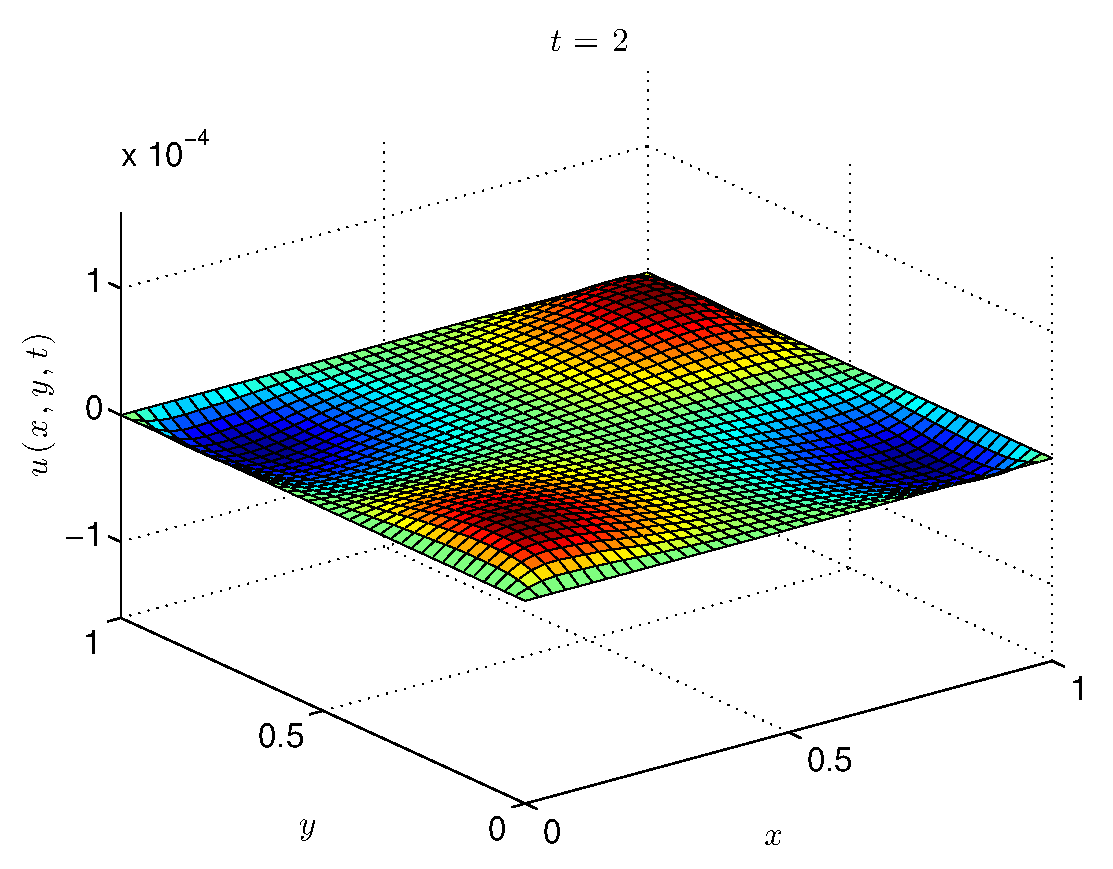
\includegraphics[scale=0.6]{heat2d4} \end{center}
\end{enumerate}


%%%%%%%%%%%%%%%%%%%%%%%%%%%%%%%%%%%%%%%%%%%%%%%%%%%%%%%%%%%%%%%%%%%%%%%%%%%%%%%%

\ifthenelse{\boolean{showsols}}{\begin{solution}
\begin{enumerate}
\item We seek a solution $u(x,y,t)$ of the form
\[ u(x,y,t) = \sum_{j=1}^\infty \sum_{k=1}^\infty a_{j,k}(t) \psi_{j,k} (x,y),\]
given a forcing function of the form
\[ f(x,y,t) = \sum_{j=1}^\infty \sum_{k=1}^\infty c_{j,k}(t) \psi_{j,k} (x,y).\]
Substituting these formulas into the differential equation $u_t = u_{xx}+ f$ yields
\begin{eqnarray*} 
  \sum_{j=1}^\infty \sum_{k=1}^\infty a'_{j,k}(t) \psi_{j,k} (x,y)
    &=& 
  \sum_{j=1}^\infty \sum_{k=1}^\infty a_{j,k}(t) \psi''_{j,k} (x,y) +
                    + \sum_{j=1}^\infty \sum_{k=1}^\infty c_{j,k}(t) \psi_{j,k} (x,y) \\[.5em]
  &=& \sum_{j=1}^\infty \sum_{k=1}^\infty -\lambda_{j,k} a_{j,k}(t) \psi_{j,k} (x,y) 
                    + \sum_{j=1}^\infty \sum_{k=1}^\infty c_{j,k}(t) \psi_{j,k} (x,y)
\end{eqnarray*}
Take an inner product of both sides with $\psi_{m,n}$ and use the orthonormality of the
eigenfunctions to obtain the ordinary differential equation
\[ a'_{m,n}(t) = -\lambda_{m,n} a_{m,n}(t) + c_{m,n}(t).\]
This differential equation is accompanied by the initial condition on $a_{m,n}(0)$ obtained
from the initial data for the problem,
\[ a_{m,n}(0) = (u_0, \psi_{m,n}) = \int_0^1 \int_0^1 2 u_0(x,y) \sin(m \pi x) \sin(n \pi y)\,\dop x\,\dop y.\]
The contribution from $c_{m,n}(t)$ can be computed \emph{a priori} from the expansion of the
forcing data in the eigenfunctions, i.e.,
\[ c_{m,n}(t) = (f(x,y,t), \psi_{m,n}(x) ) = \int_0^1 \int_0^1 2 f(x,y,t) \sin(m \pi x) \sin(n \pi y)\,\dop x\,\dop y.\]


\item Since $u_0(x) = 0$ for all $x\in[0,1]$, we simply have $a_{m,n}(0)=0$.
     
   The computation of $c_{m,n}(t)$ requires a bit more work.  We heed to compute 
\begin{eqnarray*}
    c_{m,n}(t) &=& \int_0^1 \int_0^1 2 f(x,y,t) \sin(m \pi x) \sin(n \pi y)\,\dop x\,\dop y \\[0.25em]
               &=& \int_0^1 \int_0^1 2 (x-1/2)^3(y-1/2)@\eop^{-t}\sin(m \pi x) \sin(n \pi y)\,\dop x\,\dop y \\[0.25em]
               &=& \eop^{-t} \int_0^1 \int_0^1 2 (x-1/2)^3(y-1/2)\sin(m \pi x) \sin(n \pi y)\,\dop x\,\dop y.
\end{eqnarray*}
The integral can be computed using symbolic integration.  From Mathematica, we find that
\[ \int_0^1 \int_0^1 2 (x-1/2)^3(y-1/2)\sin(m \pi x) \sin(n \pi y)\,\dop x\,\dop y
     = {(1+(-1)^m)(1+(-1)^n) (m^2\pi^2-24)\over 8 m^3 n \pi^4},\]
giving 
\[ c_{m,n}(t) = {(1+(-1)^m)(1+(-1)^n) (m^2\pi^2-24)\over 8 m^3 n \pi^4} \eop^{-t}.\]
The differential equation $a_{m,n}'(t) = -\lambda_{m,n} a_{m,n}(t) + c_{m,n}(t)$ 
has the exact solution
\[ a_{m,n}(t) 
    = \eop^{-\lambda_{m,n}t} a_{m,n}(0) + \int_0^t \eop^{-\lambda_{m,n}(t-\tau)} c_{m,n}(\tau)\,\dop \tau
    = \int_0^t \eop^{-\lambda_{m,n}(t-\tau)} c_{m,n}(\tau)\,\dop \tau,\]
where the last equality holds for the initial condition $u_0(x,y)= 0$ for all $x,y\in[0,1]$.
Notice that
\[ \int_0^t \eop^{-\lambda_{m,n}(t-\tau)} \eop^{-\tau}\,\dop \tau
    = \eop^{-\lambda_{m,n}t} \Big[{\eop^{(\lambda_{m,n}-1)\tau}\over \lambda_{m,n}-1}\Big]_{\tau=0}^{\tau=t}
    = \eop^{-\lambda_{m,n}t} {\eop^{(\lambda_{m,n}-1)t}-1\over \lambda_{m,n}-1}
    = {\eop^{-t} - \eop^{\lambda_{m,n}t}\over \lambda_{m,n}-1}.
\] 
Hence, we have
\[ \int_0^t e^{-\lambda_{m,n}(t-\tau)} c_{m,n}(\tau)\, \dop \tau
    = \Big({(1+(-1)^m)(1+(-1)^n) (m^2\pi^2-24)\over 8 m^3 n \pi^4}\Big)
     \Big( {\eop^{-t} - \eop^{-\lambda_{m,n} t} \over \lambda_{m,n}-1}\Big).\]
Finally, we can simplify the true solution as
\[ u(x,t) = \sum_{m=1}^\infty \sum_{n=1}^\infty 
    \Big({(1+(-1)^m)(1+(-1)^n) (m^2\pi^2-24)\over 8 m^3 n \pi^4}\Big)
    \Big( {\eop^{-t} - \eop^{-\lambda_{m,n} t} \over \lambda_{m,n}-1}\Big)
    \big(2\sin(m\pi x)\sin(n\pi y)\big).\]
    
 
\item Plots at the requested times are shown below, followed by the code that
generated them.

{[GRADERS: If students do not simplify the exponentials as given in the formula
for $u(x,t)$ above, it is possible that errors will prevent an accurate plot 
for the later times below.  For example, it could be that $e^{\lambda_{m,n}t}$
evaluates in MATLAB as {\tt Inf}, while $e^{-\lambda_{m,n}t}$ evaluates as
{\tt 0}, with ${\tt Inf}\times {\tt 0} = {\tt NaN}$, an unplottable quantity.
Please deduct 5~points (once) if this is a problem for any of the plots.]}

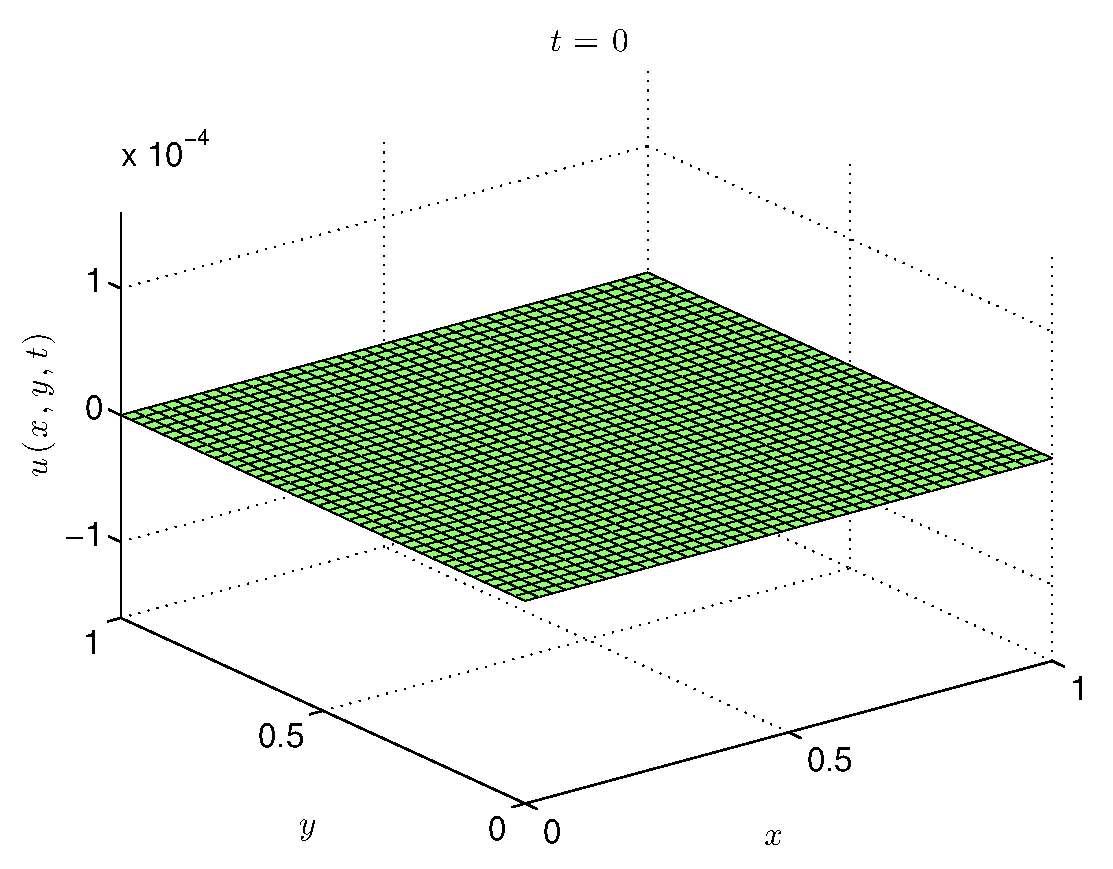
\includegraphics[scale=0.4]{heat2d1}
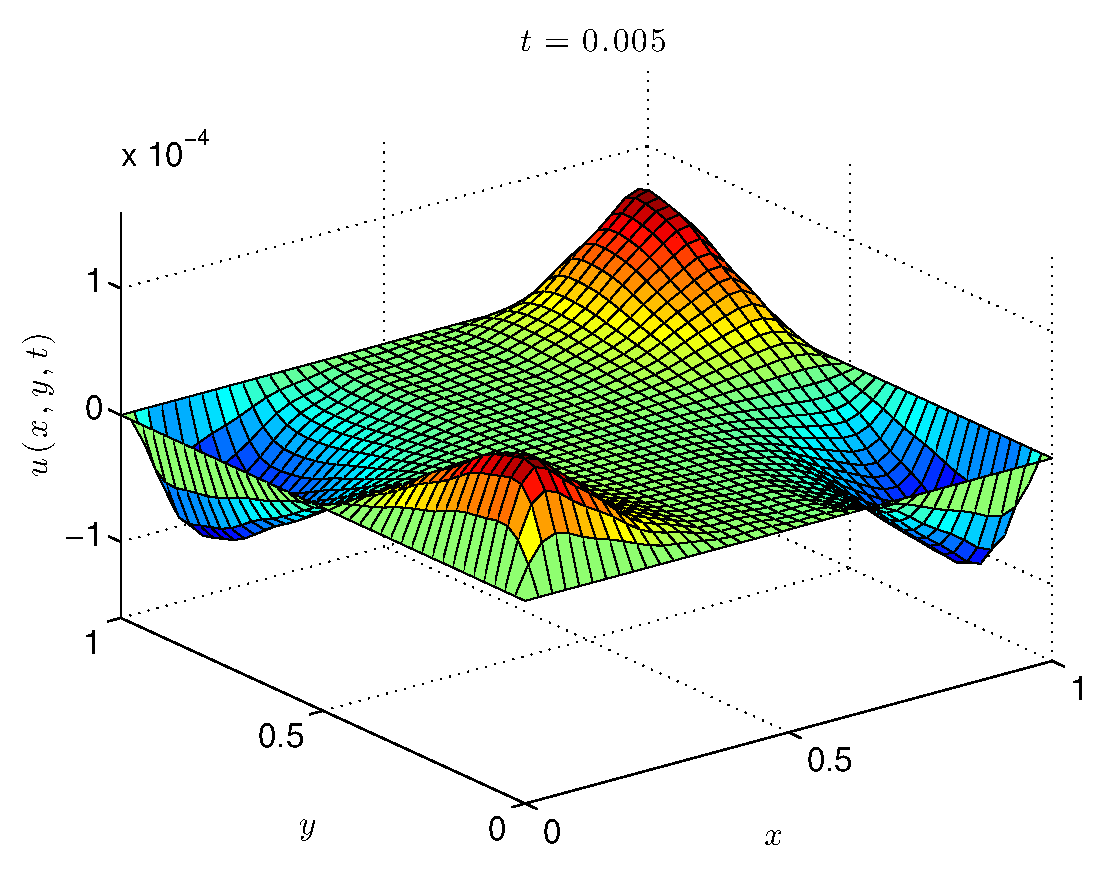
\includegraphics[scale=0.4]{heat2d2}

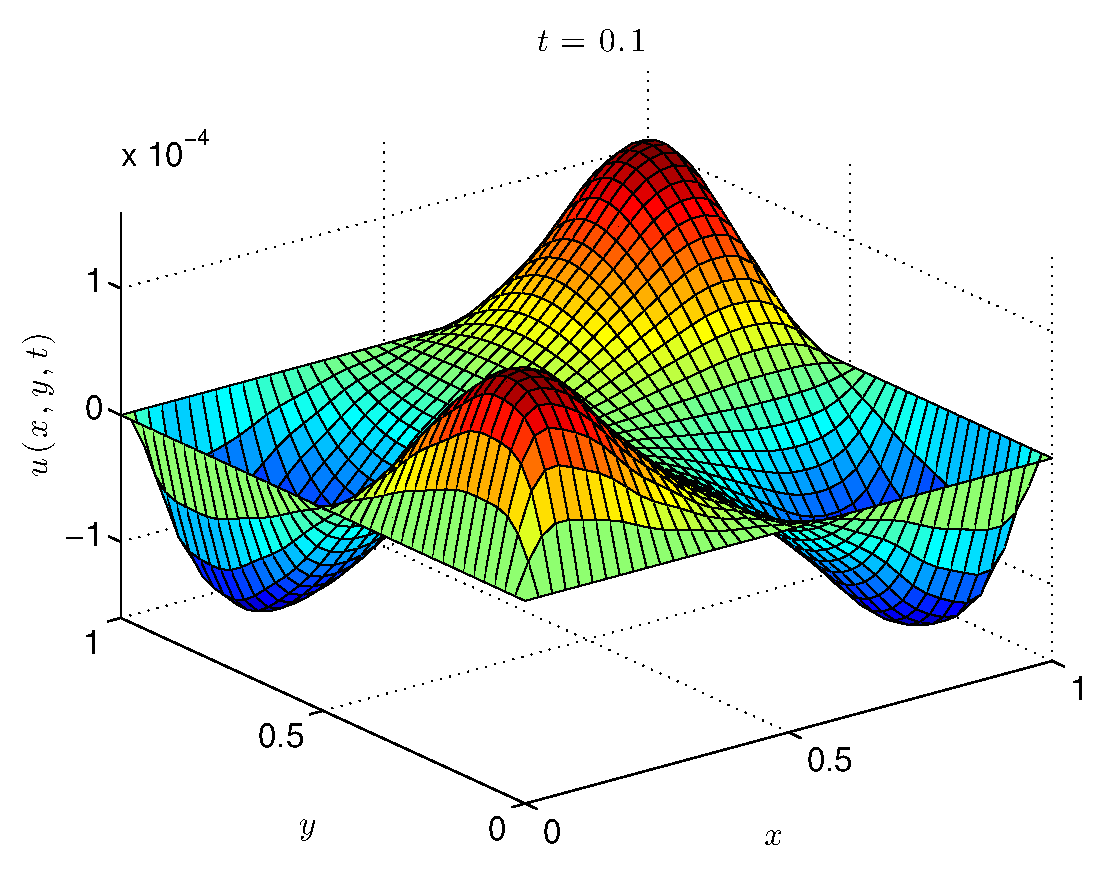
\includegraphics[scale=0.4]{heat2d3}
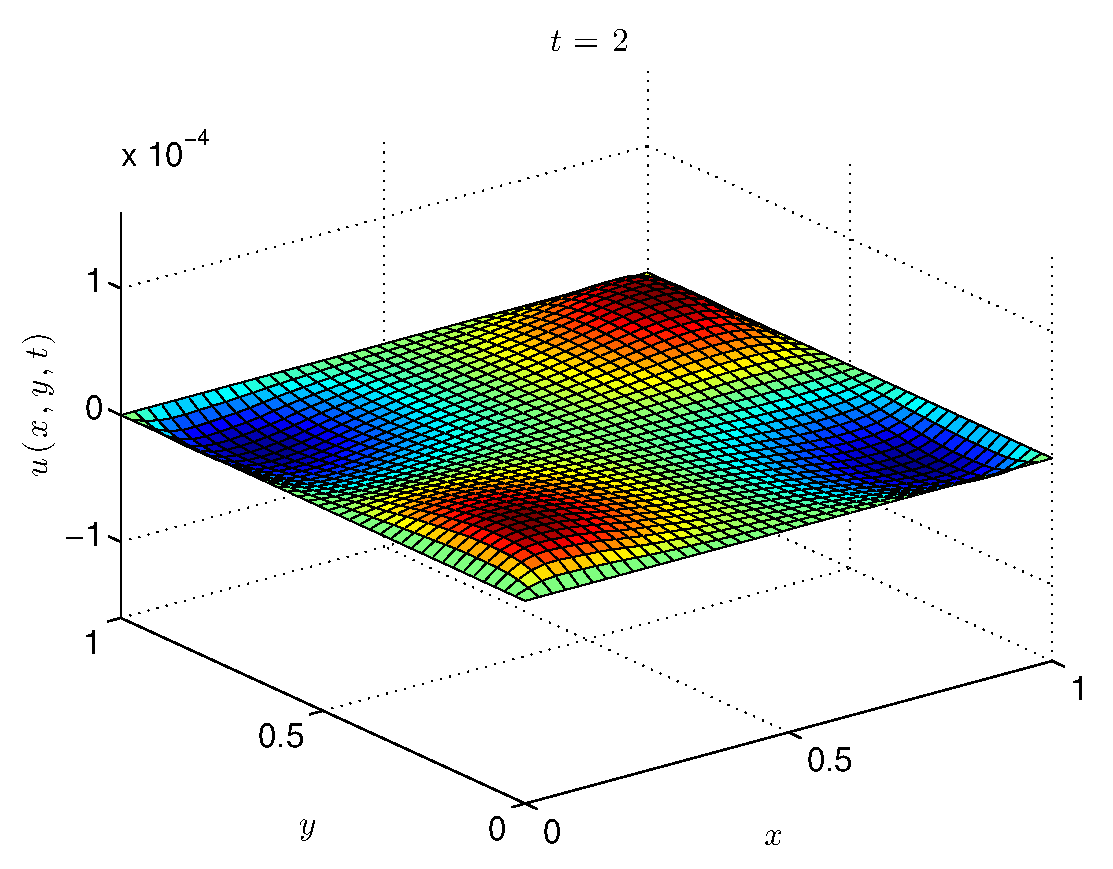
\includegraphics[scale=0.4]{heat2d4}

\input heat2dcode
\end{enumerate}
\end{solution}}{}

